% Drawing 43/03-12 -- folder 43, batch 03, archive page 52 (PDF page 53).
% Transcription: en haut à droite, un croquis en escalier : dans l'angle inférieur gauche d'un cadre, des cases empilées en trois colonnes de hauteurs décroissantes ; une flèche descendante au-dessus de la première colonne, une flèche vers la gauche le long du bas ; de petits coins tracés à l'intérieur du cadre.
% Kind: staircase of boxes in the corner of a frame. Method 2 (schematic redraw from the facsimile). Status: ok.
% Notes: Ink. A frame (left side, top in two strokes, right side, a doubled bottom stroke); in its lower left corner a staircase of boxes: three in the first column, two in the second, one in the third; an arrow pointing down onto the first column and an arrow pointing left along the bottom; three small corner marks inside the frame. The two struck schemas at the upper left of the page (the gothic p, m with primes under a bracket) are text, struck, and not drawn. Still differs: the number of boxes in each column (3, 2, 1) is a reading of overdrawn strokes, and the corner marks are placed by eye. Redrawn 2026-11-12 (issue 128): to check again. 2026-11-13, Claude Opus 5.5, overlay check (issue 147): re-read on millimetre grids of the 228 ppi scan (rendered at 350 dpi in colour); not compiled (no TeX engine in the session), the TikZ was rasterised by a script and laid over the crop; every stroke now lies on its ink to within about 1 unit. Changed: all strokes moved by 1 to 2 units onto their ink (the frame's left side and the boxes stood to the right of it); the boxes are drawn as the strokes of the page (three rows in the first column, two in the second, one in the third, each column closed by its right side) instead of overlapping rectangles; added the short upright stroke inside the top left of the frame and the short stroke closing the bottom right corner. The count 3, 2, 1 is clear on the scan, not a reading of overdrawn strokes. Left out: a speck to the left of the frame.
% Coordinates: 1 unit = 1 mm = 1/100 of the crop width, y downwards as on the crop (bbox in page fractions: [0.54, 0.065, 0.9, 0.22]).
% Redrawn by Claude (claude-fable-5-2), issue #128, 2026-11-12; not checked by a human; not compiled (no TeX in the session).
% Rights: reproduces part of the work -- behind RENDER_TRANSCRIPTS, never published by itself.
\documentclass[tikz,border=3pt]{standalone}
\usepackage{amsmath,amssymb}
\usetikzlibrary{patterns,arrows.meta}
\tikzset{pencil/.style={black!45}, struck/.style={black!35}, mpt/.style={circle,draw,inner sep=1.3pt}, pt/.style={circle,fill,inner sep=0.9pt}, opt/.style={circle,draw,fill=white,inner sep=1.1pt}, Rd/.style={red!75!black}, Gn/.style={green!45!black}, Br/.style={brown!70!black}}
\begin{document}
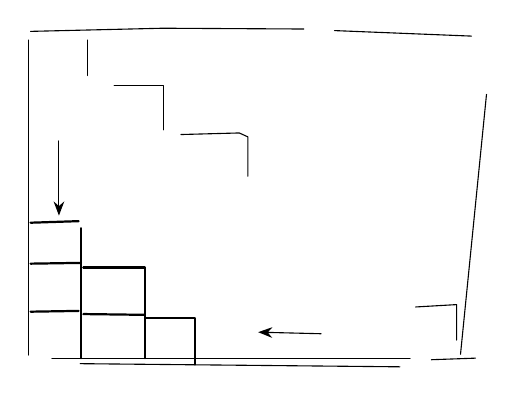
\begin{tikzpicture}[x=1mm,y=-1mm,line cap=round,line join=round,font=\small]
\draw (23.9,10.5) -- (23.9,50.5);
\draw (24.2,9.4) -- (41,9) -- (58.9,9.1);
\draw (62.8,9.3) -- (80.2,10);
\draw (31.4,10.5) -- (31.4,15);
\draw (82.1,17.4) -- (78.8,50.4);
\draw (26.9,50.9) -- (72.4,50.9);
\draw (30.5,51.6) -- (71.1,52);
\draw (75.1,51.1) -- (80.7,50.9);
\draw[thick] (24.2,33.7) -- (30.3,33.5);
\draw[thick] (24.2,38.9) -- (30.6,38.8);
\draw[thick] (24.2,45) -- (30.3,44.9);
\draw[thick] (30.6,34.4) -- (30.6,50.9);
\draw[thick] (30.9,39.4) -- (38.7,39.4) -- (38.7,50.9);
\draw[thick] (30.9,45.3) -- (38.7,45.4);
\draw[thick] (38.9,45.8) -- (45.1,45.8) -- (45.1,51.7);
\draw[-{Stealth[length=1.8mm]}] (27.8,23.3) -- (27.8,32.8);
\draw[-{Stealth[length=1.8mm]}] (61.1,47.8) -- (53.1,47.6);
\draw (34.8,16.3) -- (41.1,16.3) -- (41.1,21.9);
\draw (43.3,22.5) -- (50.7,22.3) -- (51.8,22.8) -- (51.8,27.8);
\draw (73.1,44.4) -- (78.3,44.1) -- (78.3,48.6);
\end{tikzpicture}
\end{document}
